\documentclass{beamer}
\mode<presentation> {
%\usetheme{Madrid}
%\usetheme{default}
\usepackage{color}
\definecolor{bottomcolour}{rgb}{0.21,0.11,0.21}
\definecolor{middlecolour}{rgb}{0.21,0.11,0.21}
\setbeamercolor{structure}{fg=white}
\setbeamertemplate{frametitle}[default]%[center]
\setbeamercolor{normal text}{bg=black, fg=white}
\setbeamertemplate{background canvas}[vertical shading]
[bottom=bottomcolour, middle=middlecolour, top=black]
\setbeamertemplate{items}[circle]
\setbeamertemplate{navigation symbols}{} %no nav symbols
\setbeamercolor{block title}{use=structure,fg=white,bg=structure.fg!50!red!50!blue!100!green}
\setbeamercolor{block body}{parent=normal text,use=block title,bg=block title.bg!5!white!10!bg,fg=white}
\setbeamertemplate{navigation symbols}{}
}

\usepackage{graphicx} 
\usepackage{booktabs} 
\usepackage[utf8]{inputenc}  
\usepackage[T1]{fontenc}  
\usepackage{geometry}     
%\usepackage[francais]{babel} 
\usepackage{eurosym}
\usepackage{verbatim}
\usepackage{ragged2e}
\justifying

\input{cc_beamer}

\title[FirefoxOS - Tfe Drive]{FirefoxOS - Tfe Drive} 
\author{Genma}

\begin{document}

%% Titlepage
\begin{frame}
	\titlepage
	\vfill
	\begin{center}
		\CcGroupByNcSa{0.83}{0.95ex}\\[2.5ex]
		{\tiny\CcNote{\CcLongnameByNcSa}}
		\vspace*{-2.5ex}
	\end{center}
\end{frame}

%------------------------------------------------
\begin{frame}
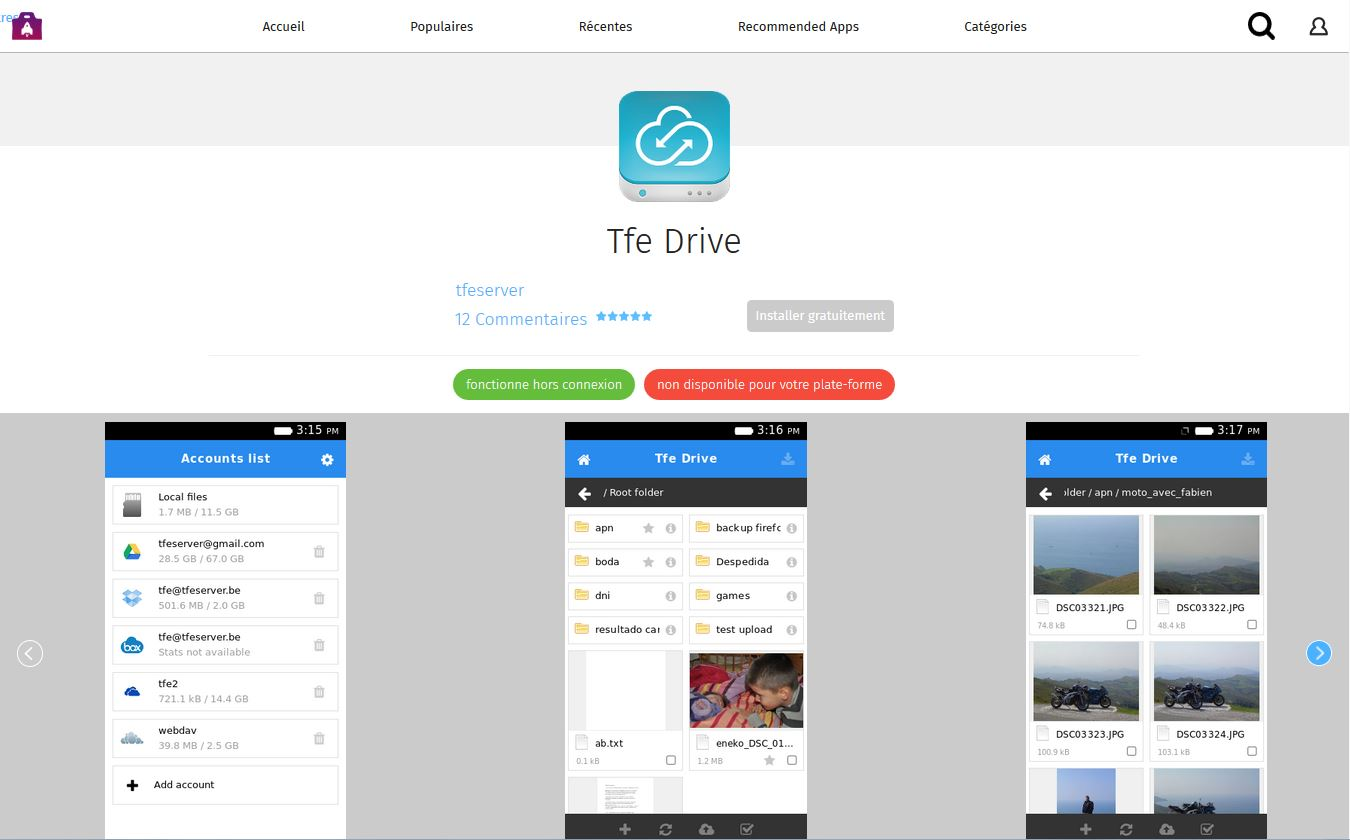
\includegraphics[scale=0.4] {./images/TFEDrive00.png} 
\end{frame}

\begin{frame}
\frametitle{Tfe Drive}
\begin{block}{Manage all your files directly from the app. Cloud and local sdcard files with the same app}
\justifying{
\begin{itemize}
\item Google Drive
\item Dropbox
\item Onedrive
\item Webdav
\item Box.com
\end{itemize}
\url{https://marketplace.firefox.com/app/tfe-drive/}
}
\end{block}

\justifying{
Synchronize your data: You can upload all the files of a directoy into the drive. Only new items will be uploaded.
This is free software. License is Apache2.0 (http://www.apache.org/licenses/LICENSE-2.0)
}
\end{frame}

\begin{frame}
\frametitle{Tfe Drive}
\begin{block}{Features}
\justifying{
\begin{itemize}
\item  open
\item  rename
\item  download to sdcard
\item  move to another folder
\item  mark/unmark starred status
\item  move to trash
\end{itemize}
}
\end{block}

\begin{block}{In each folder you can}
\justifying{
\begin{itemize}
\item create an empty directory
\item  download every files and sub folders to sdcard
\item  upload a file or sync a directory from the sdcard
\end{itemize}
}
\end{block}


\end{frame}

\begin{frame}
\begin{center}
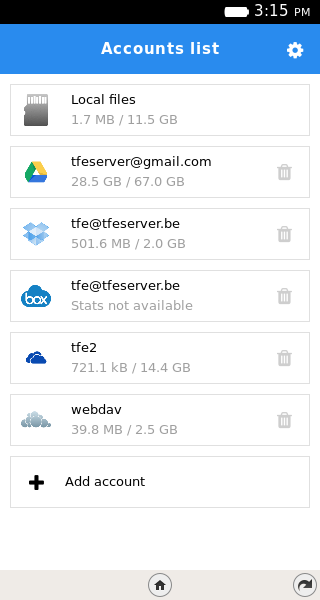
\includegraphics[scale=0.5] {./images/TFEDrive01.png} 
\end{center}
\end{frame}

\begin{frame}
\begin{center}
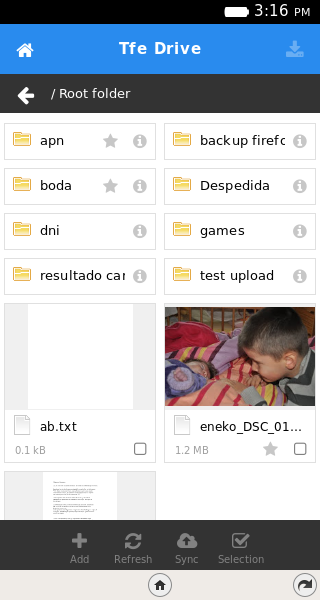
\includegraphics[scale=0.5] {./images/TFEDrive02.png} 
\end{center}
\end{frame}

\begin{frame}
\begin{center}
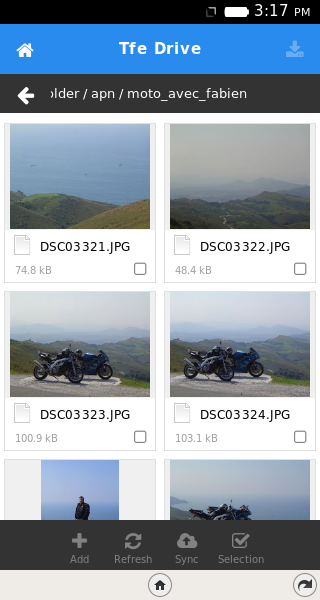
\includegraphics[scale=0.5] {./images/TFEDrive03.png} 
\end{center}
\end{frame}

\begin{frame}
\begin{center}
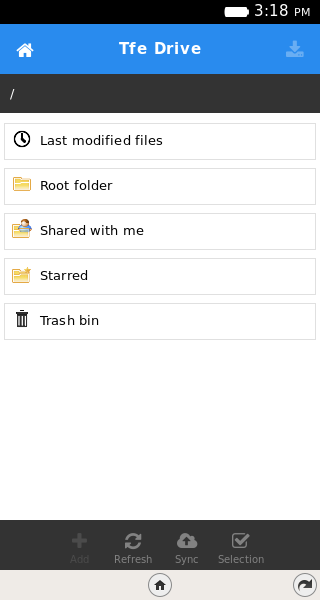
\includegraphics[scale=0.5] {./images/TFEDrive04.png} 
\end{center}
\end{frame}

\begin{frame}
\begin{center}
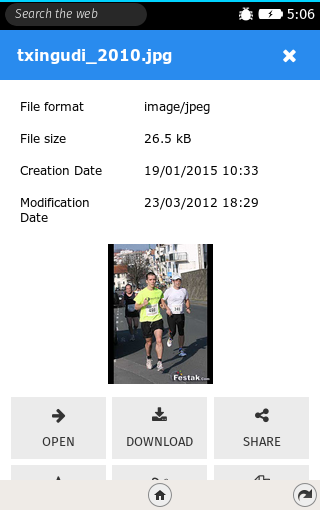
\includegraphics[scale=0.5] {./images/TFEDrive05.png} 
\end{center}
\end{frame}

\begin{frame}
\begin{center}
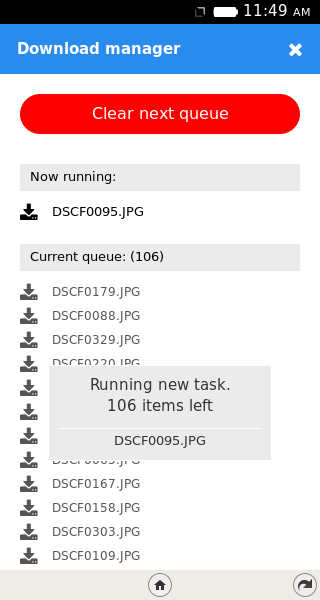
\includegraphics[scale=0.5] {./images/TFEDrive06.png} 
\end{center}
\end{frame}
\begin{frame}
\begin{center}
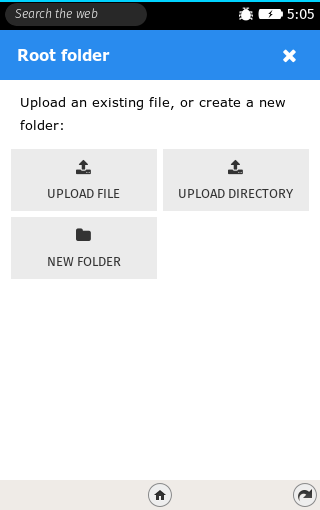
\includegraphics[scale=0.5] {./images/TFEDrive07.png} 
\end{center}
\end{frame}
\begin{frame}
\begin{center}
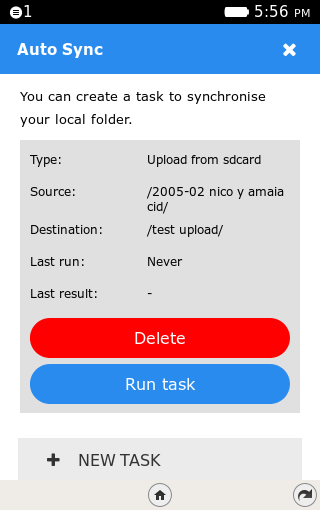
\includegraphics[scale=0.5] {./images/TFEDrive08.png} 
\end{center}
\end{frame}

\begin{frame}
\begin{center}
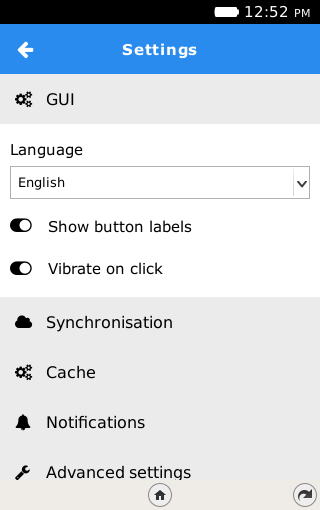
\includegraphics[scale=0.5] {./images/TFEDrive09.png} 
\end{center}
\end{frame}

\end{document}
